\clearpage
\section*{Supplementary Figures}
\setcounter{figure}{0}
\renewcommand{\figurename}{Supplementary Figure}

\begin{center}
\pandocbounded{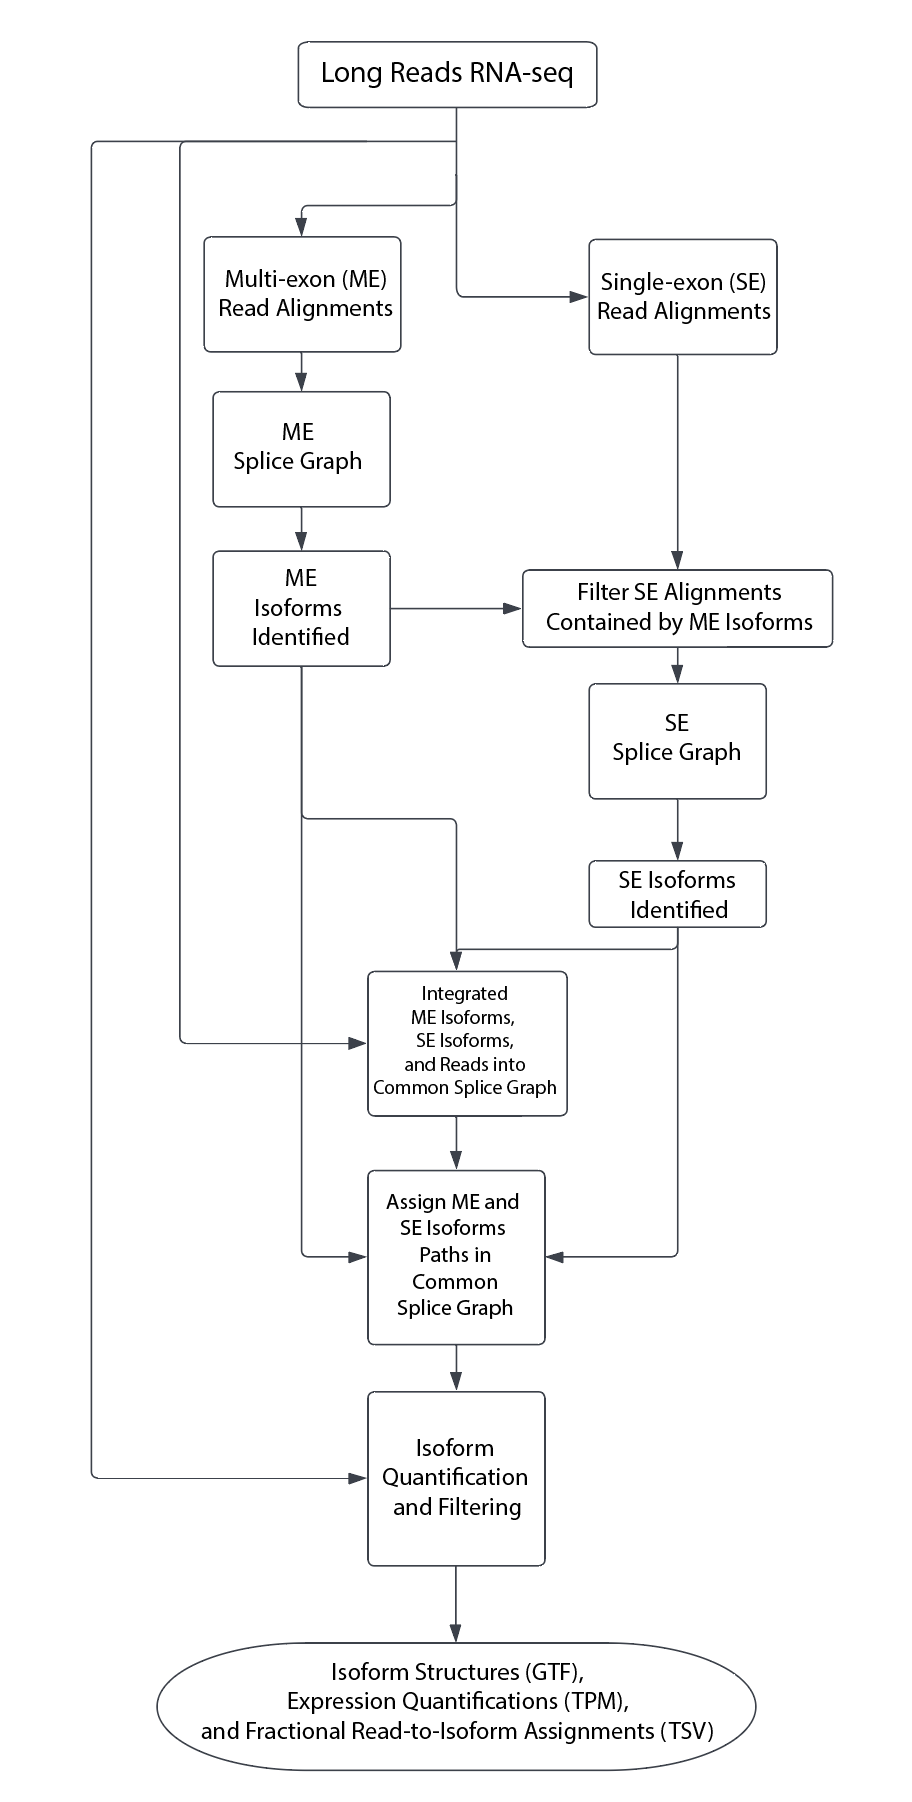
\includegraphics{figures/docx_export/SuppFig1.png}}
\end{center}

\captionof{figure}{LRAA high-level algorithm for isoform identification and quantification starting from aligned long RNA-seq reads. See \textbf{Methods} for detailed descriptions of stages.}\label{sfig:1}

\begin{center}
\pandocbounded{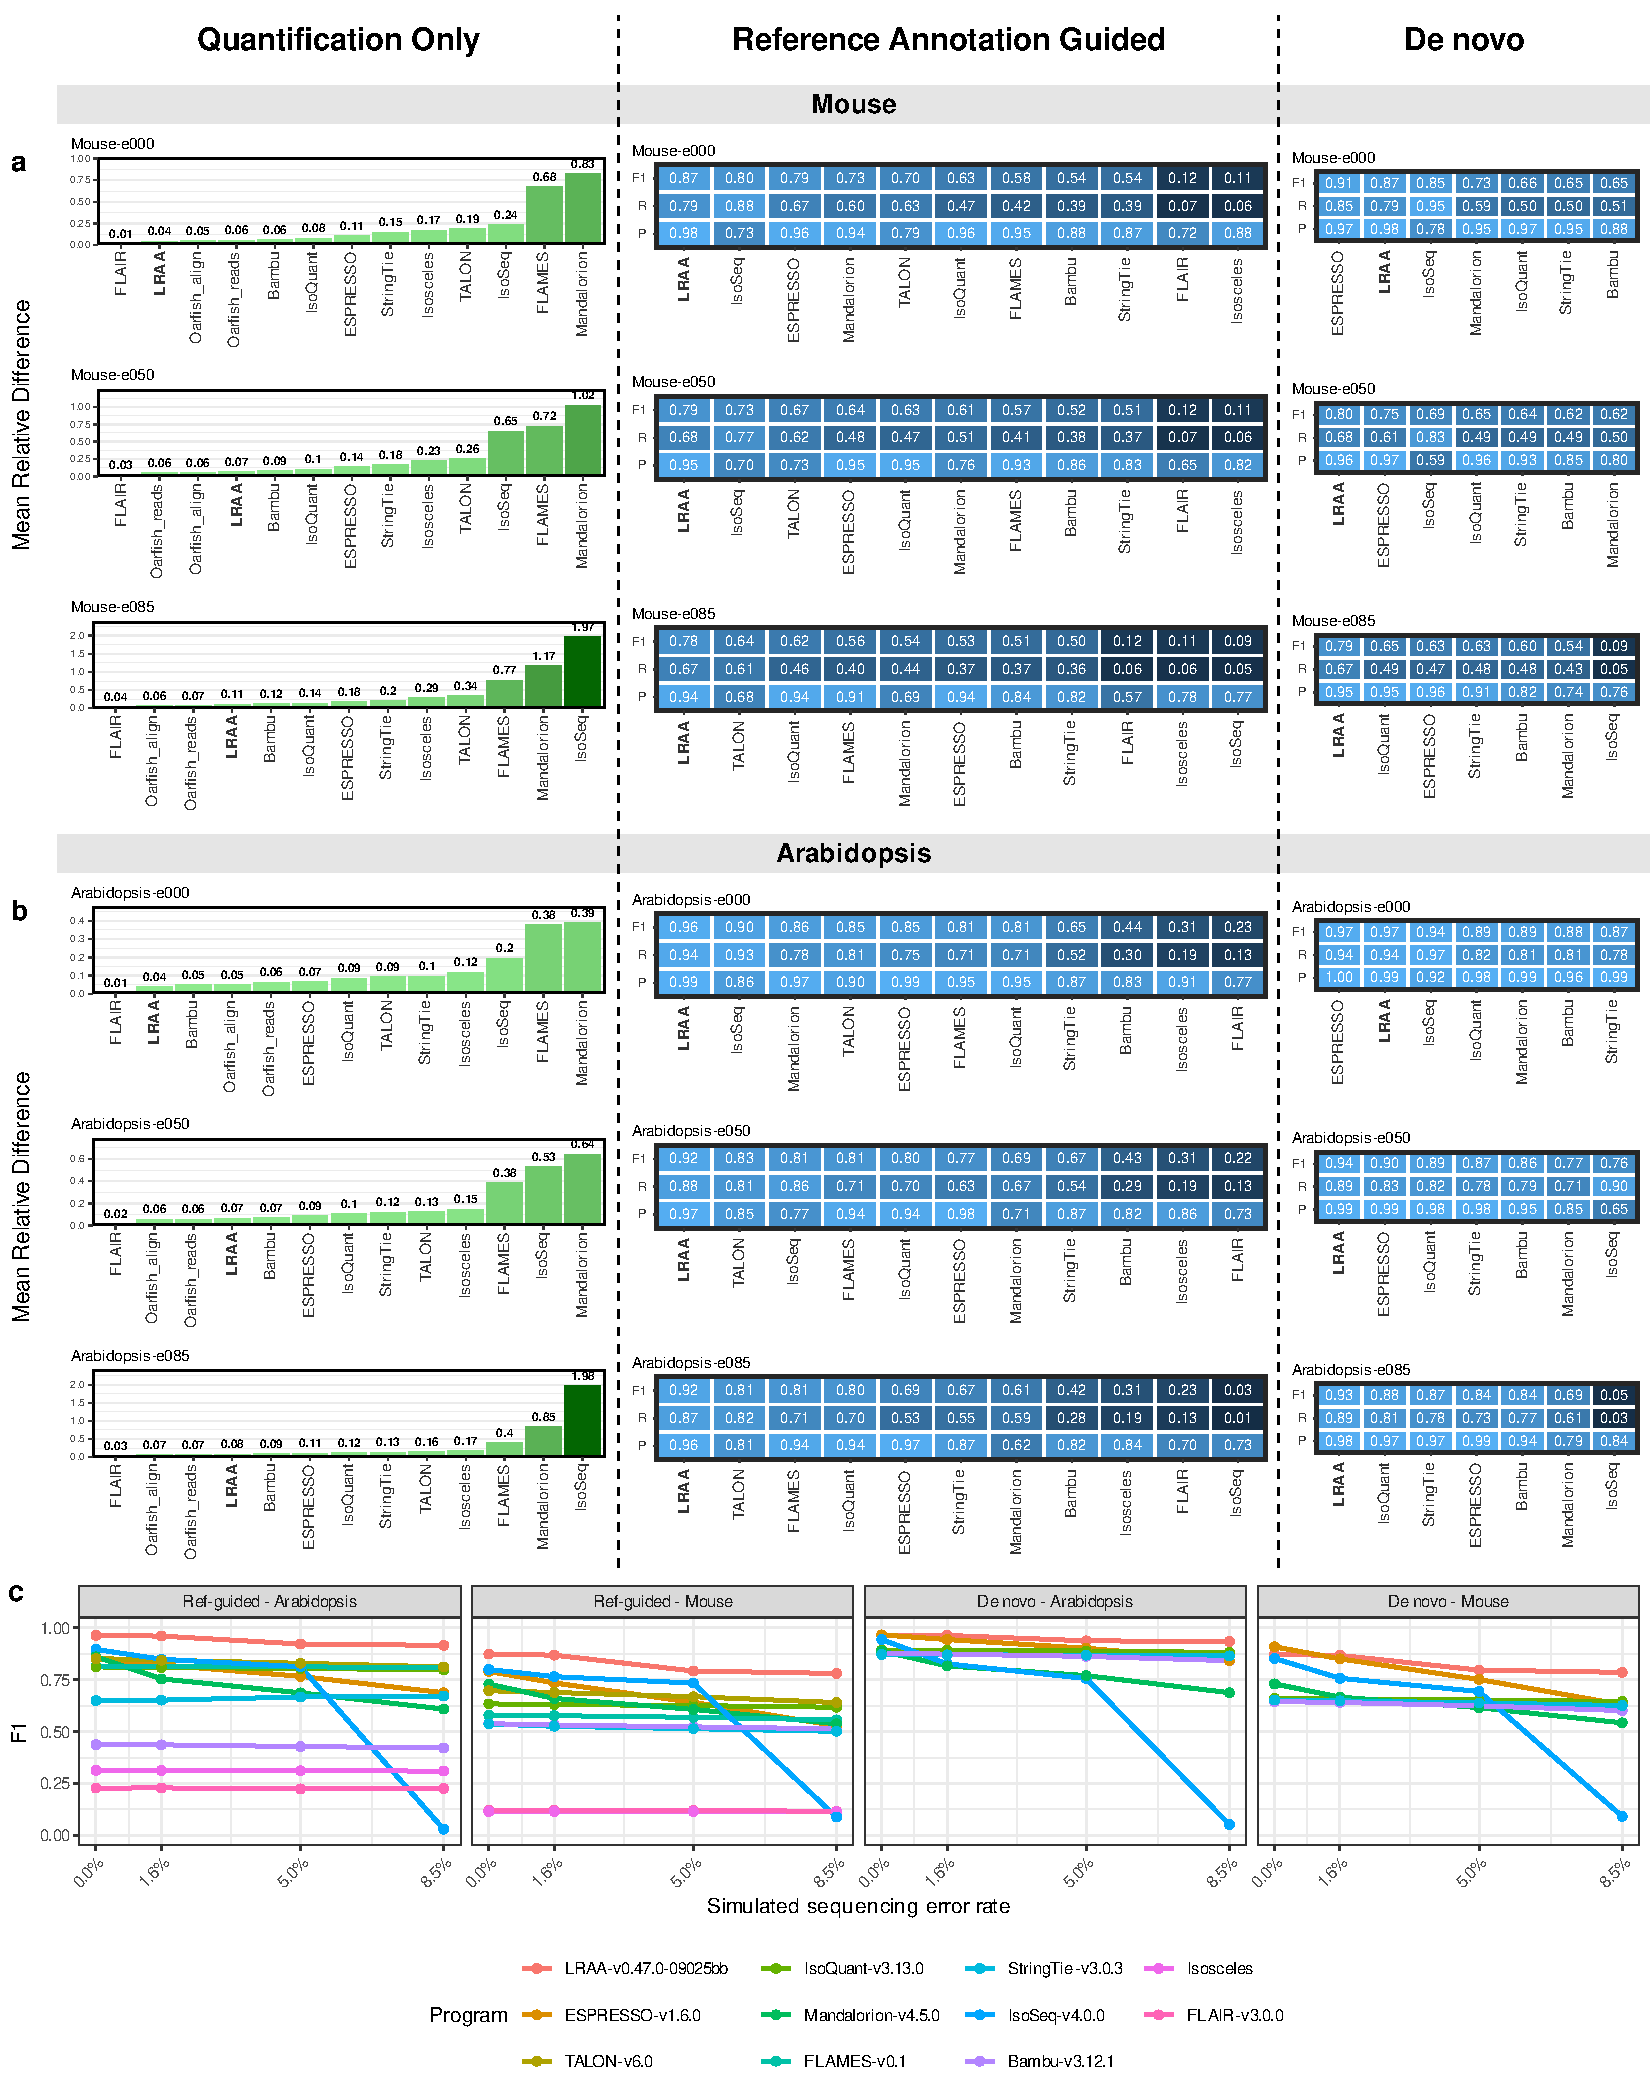
\includegraphics{figures/benchmark/SuppFig2_benchmarks_sim_error_rates.pdf}}
\end{center}

\captionof{figure}{Isoform quantification and identification accuracy based on (a) Mouse or (b) Arabidopsis simulated long RNA-seq at varied levels of sequencing error: e000: error-free, e050: 5\% error, and e085: 8.5\% error. (c) Isoform identification accuracy as a function of sequencing error according to model organism and execution mode.}\label{sfig:2}

\begin{center}
\pandocbounded{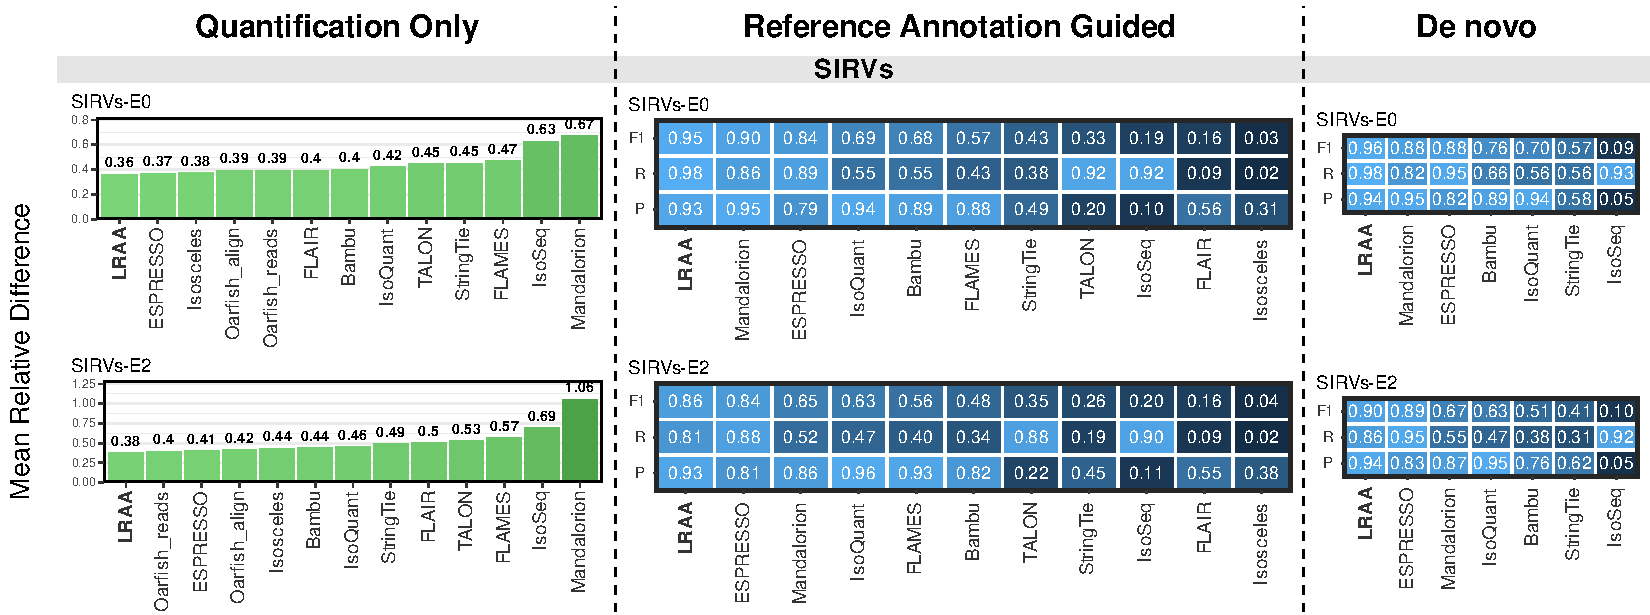
\includegraphics{figures/benchmark/SuppFig3_benchmarks_SIRVs_E0_E2.pdf}}
\end{center}

\captionof{figure}{Isoform ID and Quant accuracy for SIRV mixes E0 and E2.}\label{sfig:3}

\begin{center}
\makebox[\linewidth][l]{\sffamily\Large a}\par
\pandocbounded{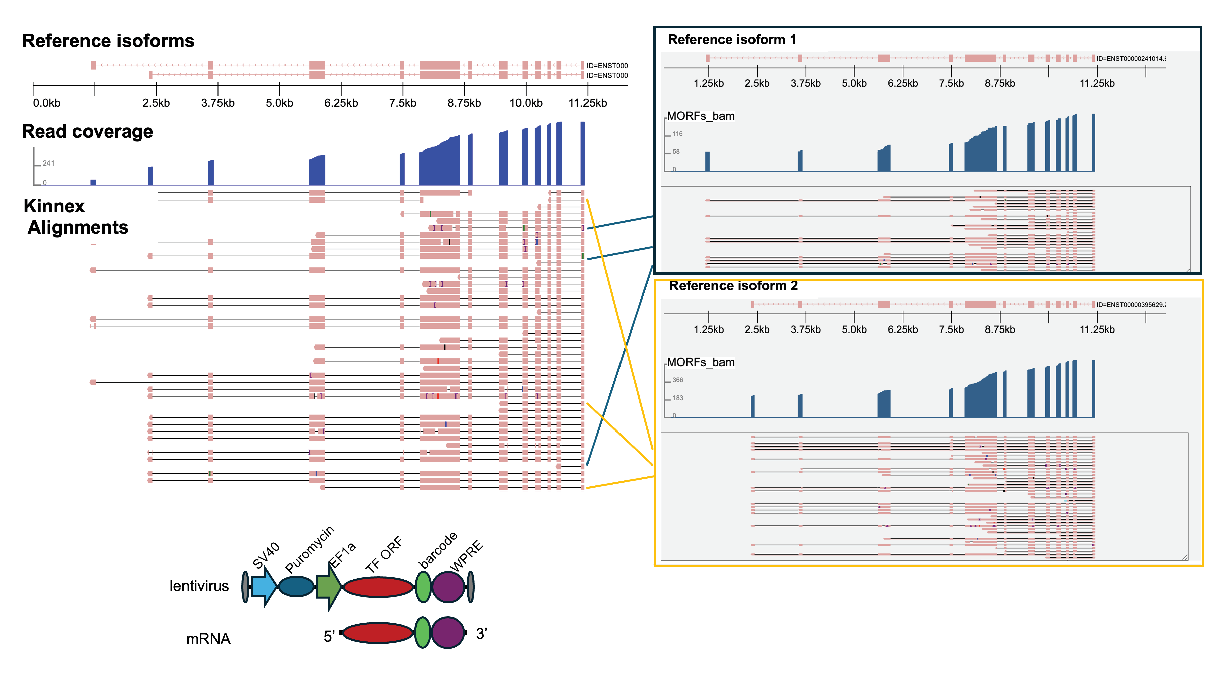
\includegraphics{figures/fixed/Supp_Fig_4-MORFsGenomeView.pdf}}

\medskip
\makebox[\linewidth][l]{\sffamily\Large b}\par
\pandocbounded{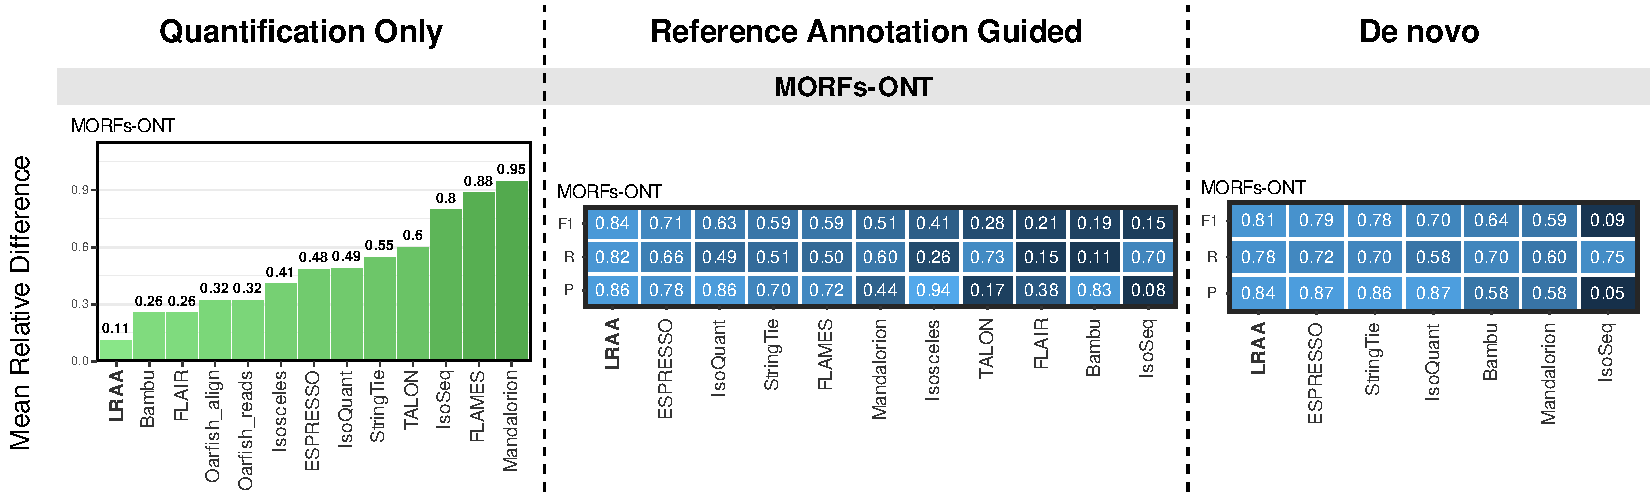
\includegraphics{figures/benchmark/SuppFig4b_benchmarks_MORFs_ONT.pdf}}
\end{center}

\captionof{figure}{Isoform ID and Quantitation using MORFs. (a) Barcoding strategy enabling unambiguous identification of isoform from which read was derived, regardless of read-to-isoform structure mapping uncertainty. MORF lentivirus construct and mRNA structures shown at bottom, adapted from \citep{joung2023}. (b) Quantification and isoform identification accuracy based on ONT long RNA-seq reads for MORFs.}\label{sfig:4}

\begin{center}
\pandocbounded{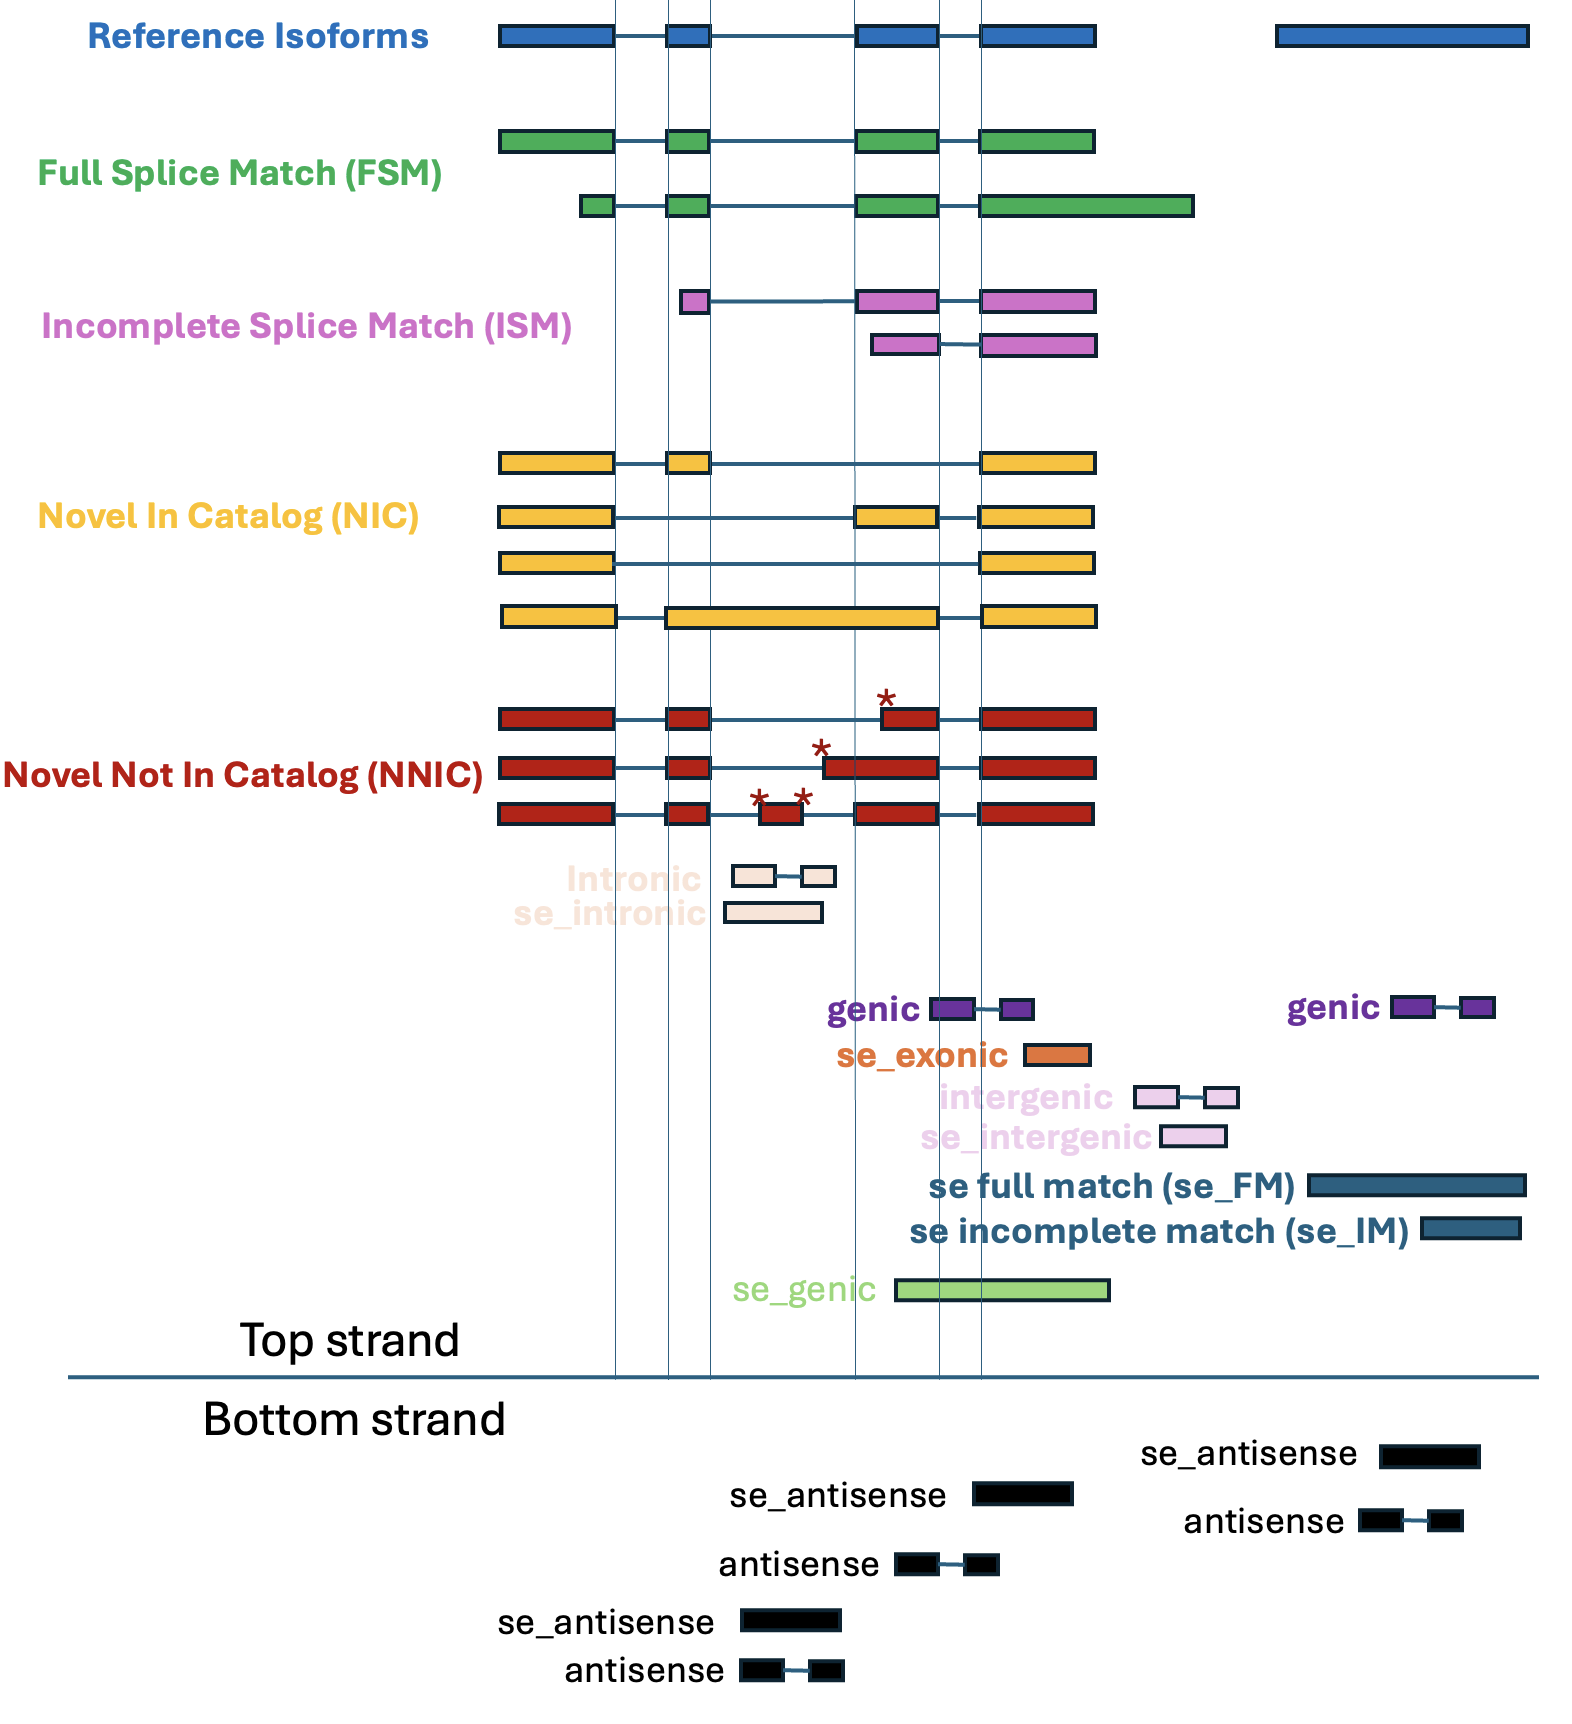
\includegraphics{figures/docx_export/SuppFig5.png}}
\end{center}

\captionof{figure}{LRAA's SQANTI-like classification scheme as applied to individual read alignments (BAM) or isoform structures (GTF) in comparison to a reference gene structure annotation (eg. GENCODE).}\label{sfig:5}

\begin{center}
\pandocbounded{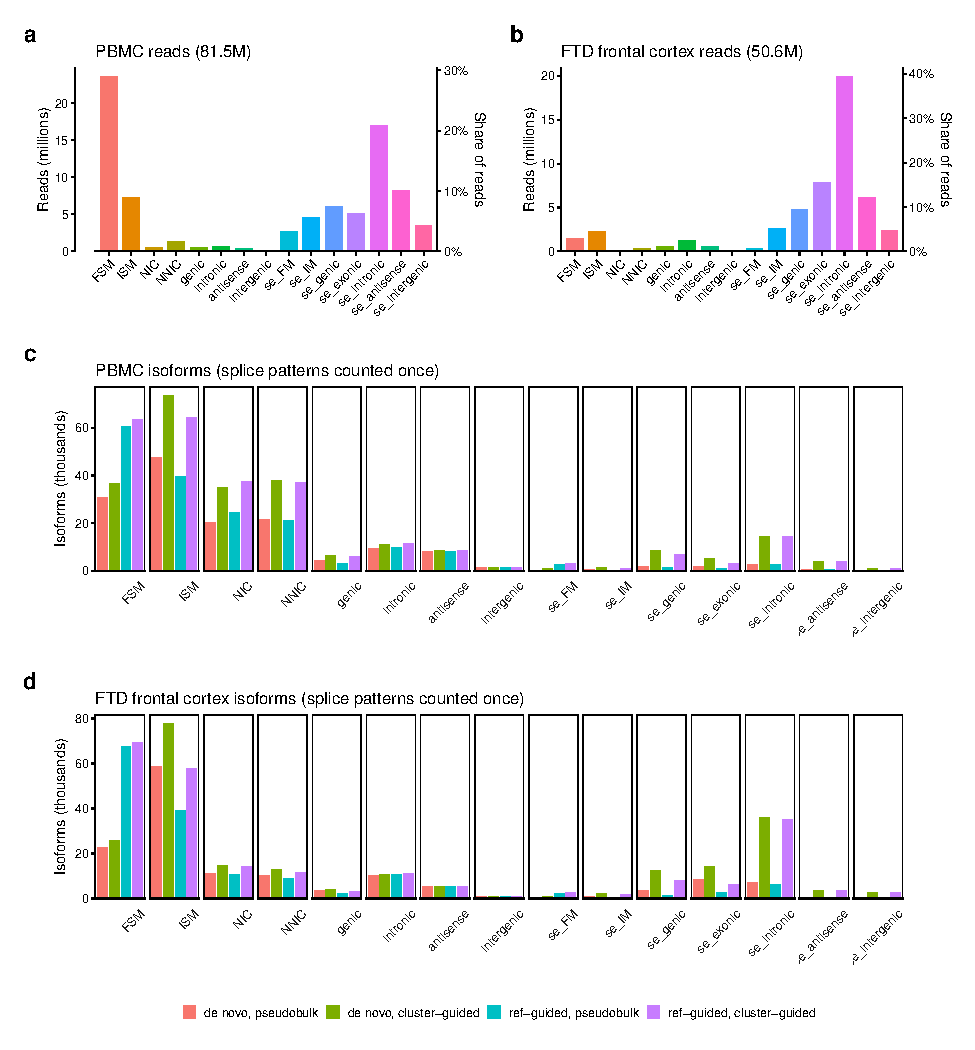
\includegraphics{figures/supp/SuppFig_categories.pdf}}
\end{center}

\captionof{figure}{SQANTI-like categories of the Kinnex reads and of the LRAA isoforms in the PBMC and FTD frontal cortex single-cell datasets. (a, b) Counts and percentages of Kinnex reads assigned to gene structures or genome regions according to LRAA SQANTI-like categories, for (a) PBMCs and (b) FTD frontal cortex. (c, d) Counts of LRAA-reconstructed isoforms from reference annotation-free (de novo) or reference annotation-guided workflows assigned to SQANTI-like categories, from the initial pseudobulk phase and the final cluster-guided phase, for (c) PBMCs and (d) FTD frontal cortex. Isoforms with identical splice patterns but different termini boundaries are counted non-redundantly as collapsed.}\label{sfig:cats}

\begin{center}
\pandocbounded{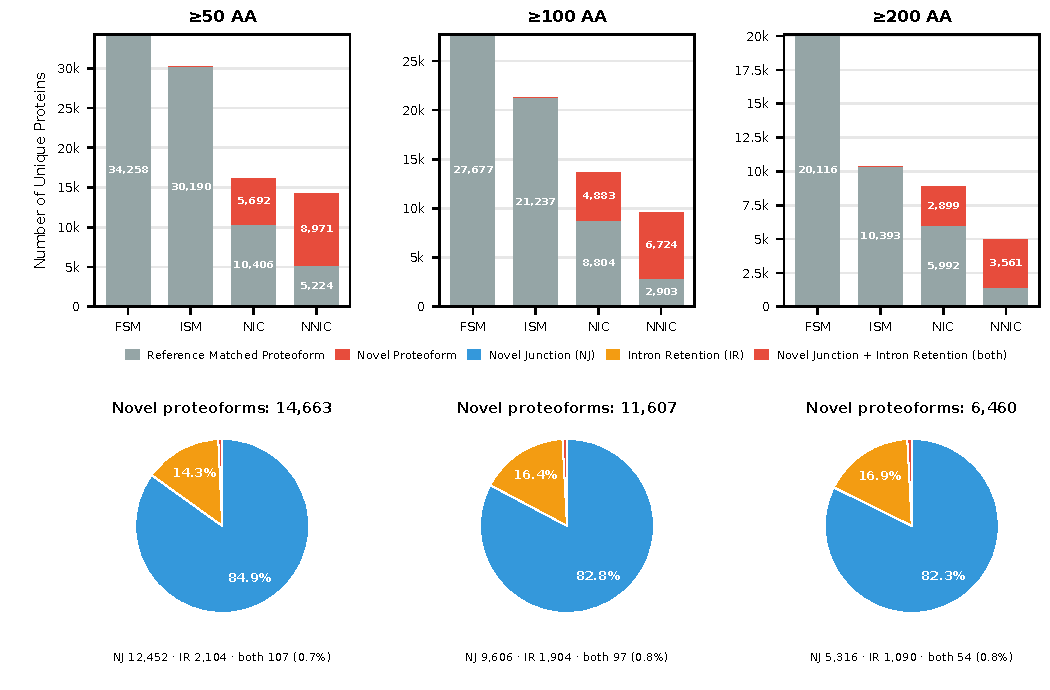
\includegraphics{figures/supp/SuppFig_proteoforms_PBMC.pdf}}
\end{center}

\captionof{figure}{Novel proteoform identification in human PBMCs. Top: Stacked bar charts showing unique protein counts by classification (FSM, ISM, NIC, NNIC) at ≥50 AA, ≥100 AA, and ≥200 AA thresholds. Proteins classified as Reference-Matched Proteoforms (gray) or Novel Proteoforms (red) based on splice junction novelty or intron retention within coding sequences. Bottom: Pie charts showing novel proteoform composition (NIC + NNIC) by splicing event type: Novel Junction only (blue), Intron Retention only (orange), or both (red); counts below each chart.}\label{sfig:6}

\begin{center}
\pandocbounded{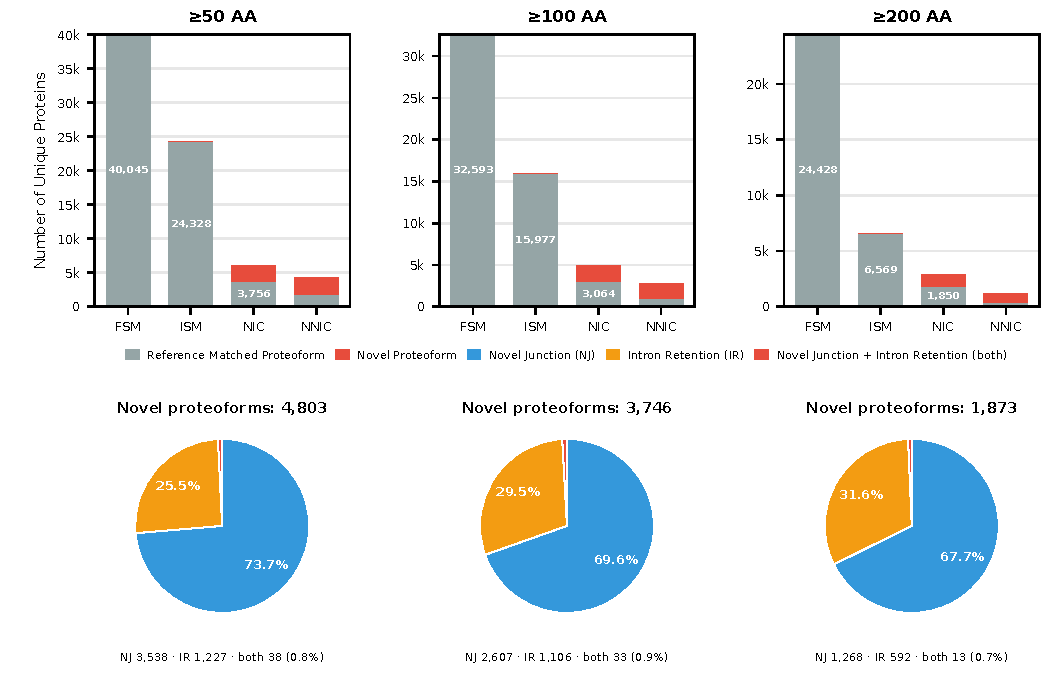
\includegraphics{figures/supp/SuppFig_proteoforms_FTD.pdf}}
\end{center}

\captionof{figure}{Novel proteoform identification in human FTD brain frontal cortex. Top: Stacked bar charts showing unique protein counts by classification (FSM, ISM, NIC, NNIC) at ≥50 AA, ≥100 AA, and ≥200 AA thresholds. Proteins classified as Reference-Matched Proteoforms (gray) or Novel Proteoforms (red) based on splice junction novelty or intron retention within coding sequences. Bottom: Pie charts showing novel proteoform composition (NIC + NNIC) by splicing event type: Novel Junction only (blue), Intron Retention only (orange), or both (red); counts below each chart.}\label{sfig:7}

\begin{center}
\pandocbounded{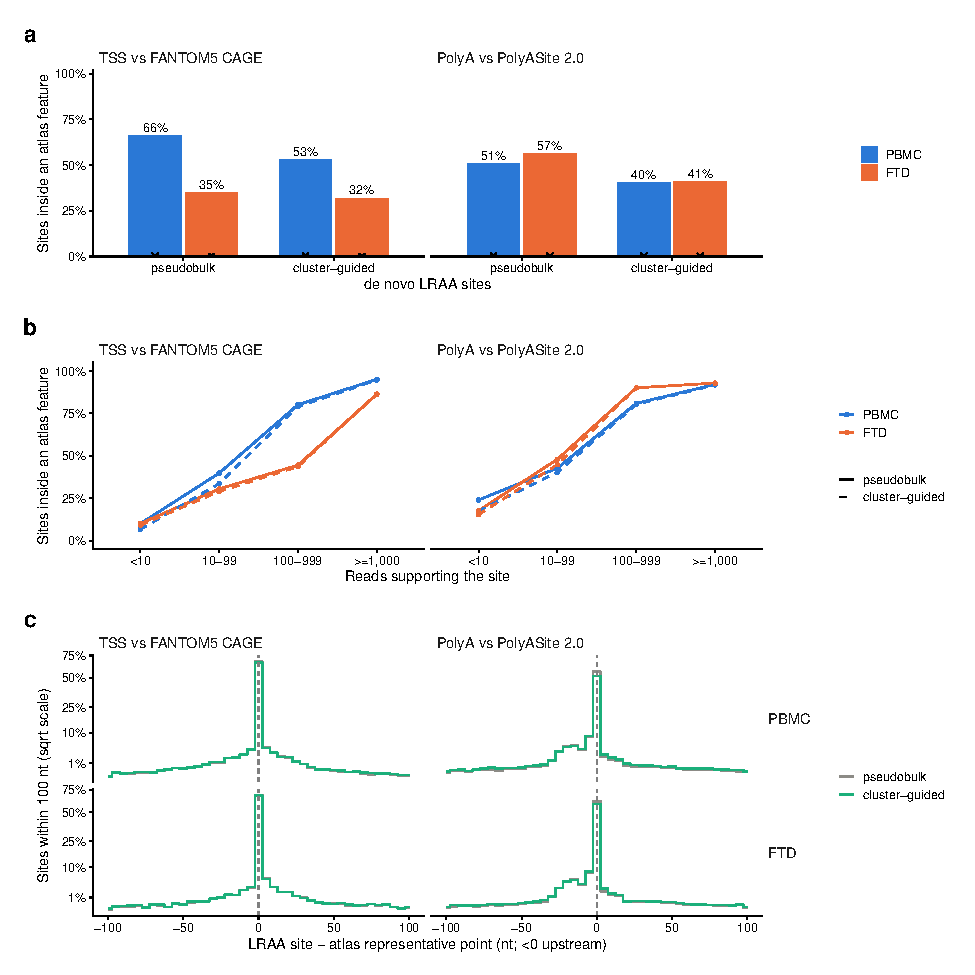
\includegraphics{figures/supp/SuppFig_site_atlas.pdf}}
\end{center}

\captionof{figure}{Agreement of LRAA's TSS and PolyA sites with FANTOM5 CAGE peaks and PolyASite~2.0 clusters in the PBMC and FTD frontal cortex datasets. Sites are those of the de novo runs (pseudobulk and cluster-guided), called from the reads alone. (a) Share of sites inside a same-strand atlas peak or cluster; crosses, the same sites placed at random within the LRAA transcript spans. (b) The same share by the number of reads supporting the site. (c) Signed offset of each site from the nearest atlas representative point (CAGE summit, PolyASite cleavage site), for sites within 100 nt, as a share of those sites per 5-nt bin (square-root scale).}\label{sfig:siteatlas}

\begin{center}
\pandocbounded{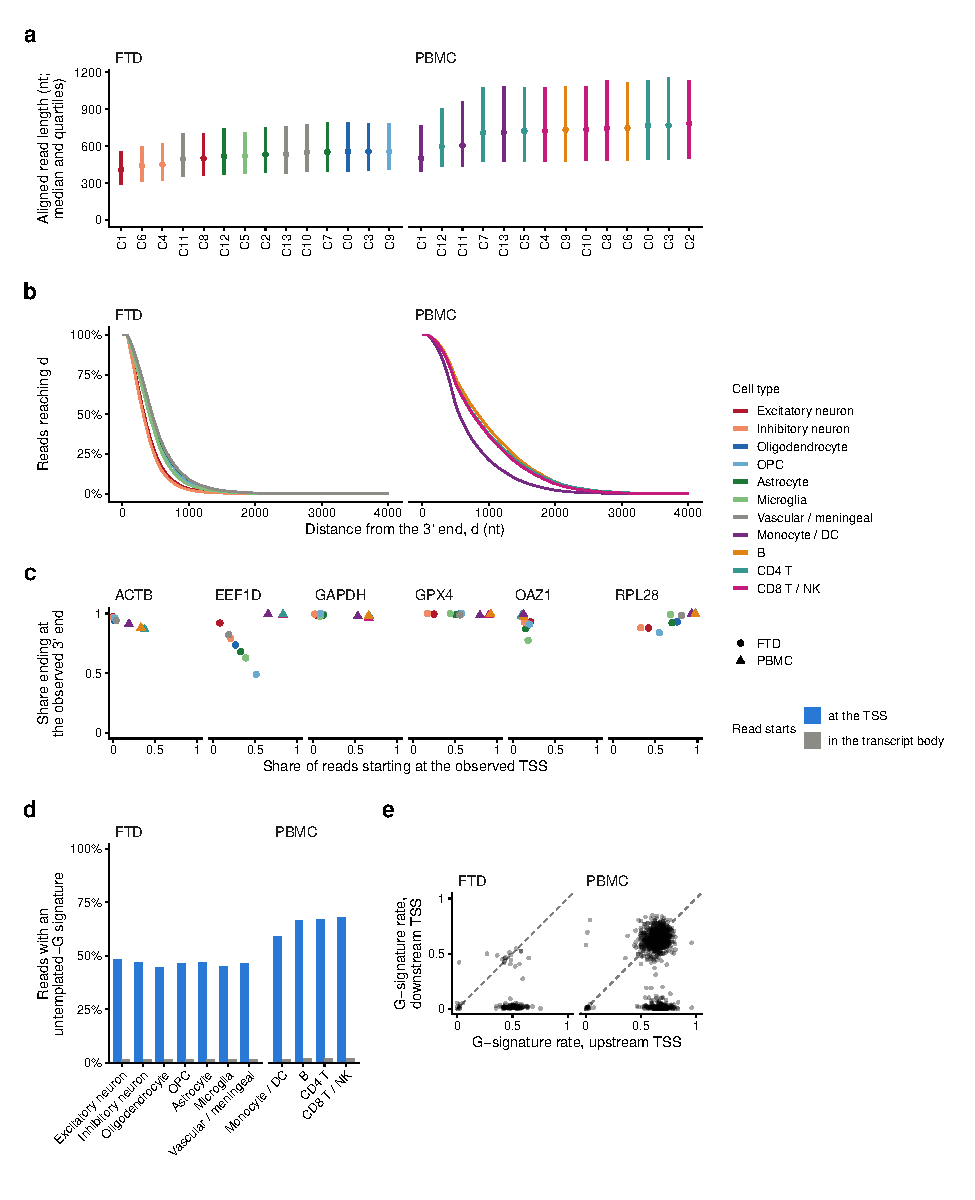
\includegraphics{figures/supp/SuppFig_TSS_5prime.pdf}}
\end{center}

\captionof{figure}{5\textquotesingle{} completeness of the reads and the untemplated-G signature, FTD frontal cortex nuclei and PBMCs. (a) Aligned read length by cluster (median and quartiles; a genome-wide sample of reads). (b) 5\textquotesingle{} completeness by cell type: the share of polyA-anchored reads reaching $d$ nt from the 3\textquotesingle{} end, averaged over genes with a single TSS. (c) Control genes: share of each cell type's reads starting at the observed TSS and ending at the observed 3\textquotesingle{} end (circles, FTD; triangles, PBMC). (d) Share of reads carrying an untemplated G at the 5\textquotesingle{} end, for reads starting at the TSS and inside the transcript body of genes with a single TSS. (e) The same signature at the upstream and downstream sites of each high-confidence TSS switch called before LRAA used the cap signature (LRAA version 0.45.0; site pairs with at least 20 informative reads at each site), counting a read as capped by LRAA's definition (\textbf{Methods}). (d, e) Reads whose genomic base upstream of the 5\textquotesingle{} end is not G. See \textbf{Methods}.}\label{sfig:tss5prime}

\clearpage
\section*{Supplementary Tables}

\noindent\textbf{Supplementary Table 1.} High-confidence differential isoform usage events between cell clusters in the PBMC and FTD frontal cortex datasets (DEXSeq on pseudo-replicates; \textbf{Methods}), one sheet per dataset and level: splice patterns, and TSS and PolyA sites tested on read ends, with each site switch's splicing class (tandem or coupled with alternative splicing) and the LRAA isoforms carrying its two sites. The FTD TSS switches are listed with a caveat: some may be 5\textquotesingle{} truncation products (\textbf{Results}). Each row is a gene and pair of clusters, with the gained and lost features, their usage, read counts and unique full-length reads in each cluster, the pairwise adjusted P values, and the switch class. A README sheet defines the columns, and a Summary sheet gives the number of genes tested, significant, with events and with high-confidence events at each level.
